% -*- mode: latex; mode: flyspell; ispell-local-dictionary: "en_US"; coding: utf-8; fill-column: 80 -*-

\documentclass{article}

\usepackage[utf8]{inputenc}
\usepackage[english]{babel}

\usepackage{amsmath,amsfonts,amssymb}
\usepackage{fullpage}
\usepackage{verbatim}

\usepackage{tikz,pgfplots}

\pgfplotsset{
  width=150mm,height=100mm,
  major grid style={thin,dotted,color=black!50},
  minor grid style={thin,dotted,color=black!50},
  grid,
  every axis/.append style={
    line width=0.5pt,
    tick style={
      line cap=round,
      thin,
      major tick length=4pt,
      minor tick length=2pt,
    },
  },
  legend cell align=left,
  legend pos=north west,
}

%%%%%%%%%%%%%%%%%%%%%%%%%%%%%%%%%%%%%%%%%%%%%%%%%%%%%%%%%%%%%%%%%%%%%%%%%%%%%%%%

\begin{document}

\title{Speicherplatzanalyse Hashmaps}
\author{}
\maketitle


% IMPORT-DATA mphf stats_mphf_size.txt
% IMPORT-DATA change smaller_tables.txt
% IMPORT-DATA hashmap stats_hashmap_size.txt


\begin{center}
	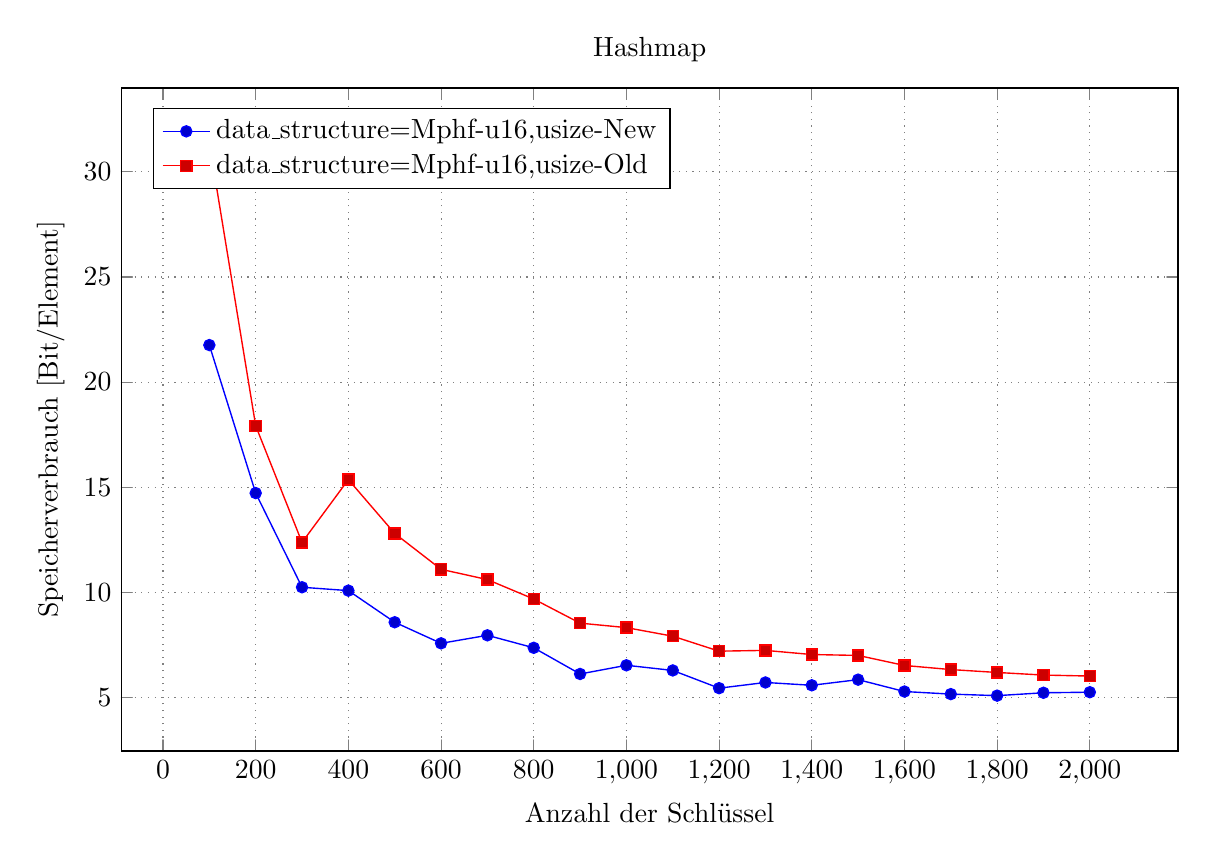
\begin{tikzpicture}
	\begin{axis}[
	title={Hashmap},
	xlabel={Anzahl der Schlüssel},
	ylabel={Speicherverbrauch [Bit/Element]},
	]
	
	%% MULTIPLOT(data_structure) SELECT size AS x, size_bytes AS y, MULTIPLOT
	%% FROM change WHERE x % 100 == 0 and x > 10 GROUP BY MULTIPLOT,x ORDER BY MULTIPLOT,x
 \addplot coordinates { (100,21.76) (200,14.72) (300,10.24) (400,10.08) (500,8.576) (600,7.57333) (700,7.95429) (800,7.36) (900,6.11556) (1000,6.528) (1100,6.28364) (1200,5.44) (1300,5.71077) (1400,5.57714) (1500,5.84533) (1600,5.28) (1700,5.15765) (1800,5.08444) (1900,5.22105) (2000,5.248) };
 \addlegendentry{data\_structure=Mphf-u16,usize-New};
 \addplot coordinates { (100,31.36) (200,17.92) (300,12.3733) (400,15.36) (500,12.8) (600,11.0933) (700,10.6057) (800,9.68) (900,8.53333) (1000,8.32) (1100,7.91273) (1200,7.2) (1300,7.23692) (1400,7.04) (1500,6.99733) (1600,6.52) (1700,6.32471) (1800,6.18667) (1900,6.06316) (2000,6.016) };
 \addlegendentry{data\_structure=Mphf-u16,usize-Old};
	
	
	
	
	
	\end{axis}
	\end{tikzpicture}
\end{center}

\begin{center}
	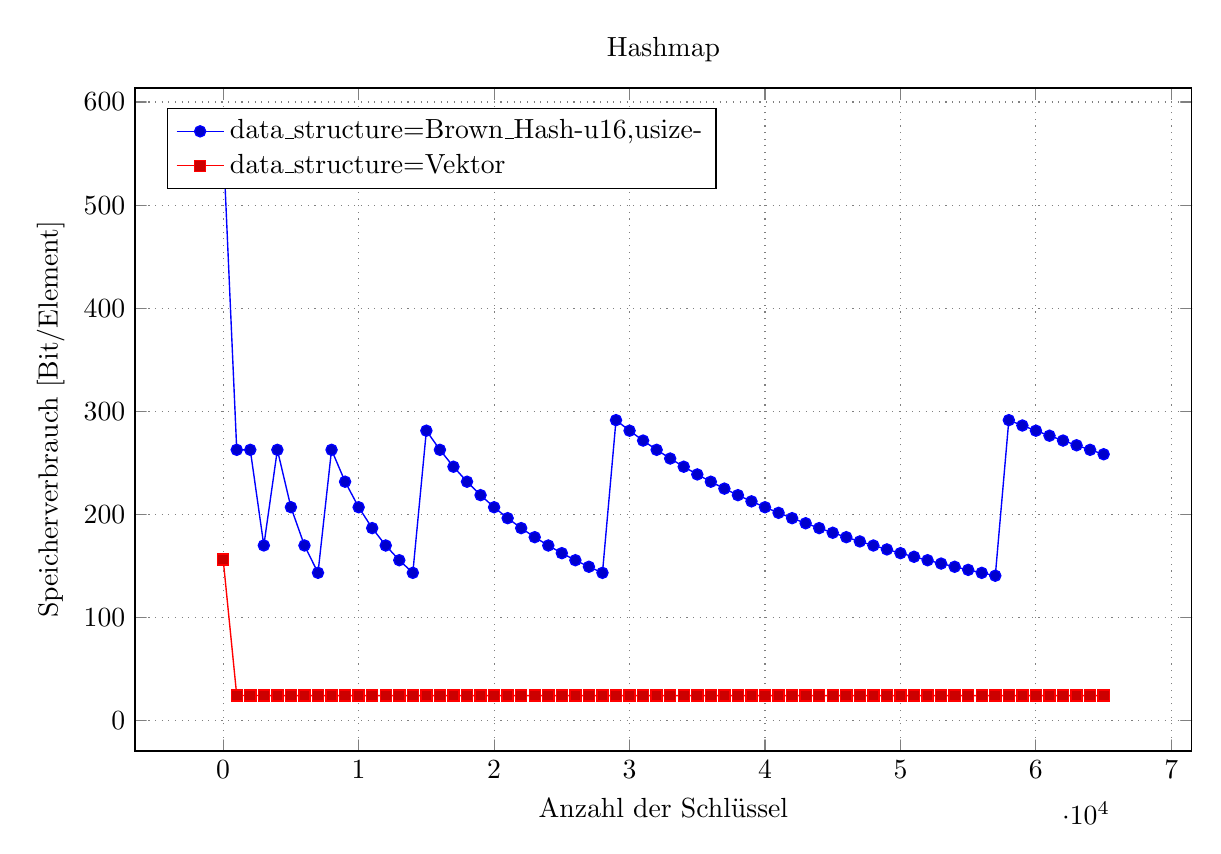
\begin{tikzpicture}
	\begin{axis}[
	title={Hashmap},
	xlabel={Anzahl der Schlüssel},
	ylabel={Speicherverbrauch [Bit/Element]},
	]
	
	%% MULTIPLOT(data_structure) SELECT size AS x, size_bytes AS y, MULTIPLOT
	%% FROM hashmap WHERE x % 1000 == 2  GROUP BY MULTIPLOT,x ORDER BY MULTIPLOT,x
 \addplot coordinates { (2,560.0) (1002,262.547) (2002,262.537) (3002,169.753) (4002,262.533) (5002,206.848) (6002,169.719) (7002,143.196) (8002,262.53) (9002,231.589) (10002,206.835) (11002,186.581) (12002,169.702) (13002,155.42) (14002,143.177) (15002,281.095) (16002,262.529) (17002,246.147) (18002,231.585) (19002,218.556) (20002,206.829) (21002,196.219) (22002,186.574) (23002,177.767) (24002,169.694) (25002,162.267) (26002,155.411) (27002,149.063) (28002,143.168) (29002,291.34) (30002,281.096) (31002,271.513) (32002,262.529) (33002,254.089) (34002,246.146) (35002,238.656) (36002,231.583) (37002,224.892) (38002,218.553) (39002,212.539) (40002,206.826) (41002,201.391) (42002,196.215) (43002,191.28) (44002,186.57) (45002,182.068) (46002,177.763) (47002,173.64) (48002,169.69) (49002,165.9) (50002,162.262) (51002,158.767) (52002,155.406) (53002,152.172) (54002,149.058) (55002,146.057) (56002,143.163) (57002,140.371) (58002,291.341) (59002,286.132) (60002,281.096) (61002,276.226) (62002,271.513) (63002,266.949) (64002,262.528) (65002,258.243) };
 \addlegendentry{data\_structure=Brown\_Hash-u16,usize-};
 \addplot coordinates { (2,156.0) (1002,24.2635) (2002,24.1319) (3002,24.0879) (4002,24.066) (5002,24.0528) (6002,24.044) (7002,24.0377) (8002,24.033) (9002,24.0293) (10002,24.0264) (11002,24.024) (12002,24.022) (13002,24.0203) (14002,24.0189) (15002,24.0176) (16002,24.0165) (17002,24.0155) (18002,24.0147) (19002,24.0139) (20002,24.0132) (21002,24.0126) (22002,24.012) (23002,24.0115) (24002,24.011) (25002,24.0106) (26002,24.0102) (27002,24.0098) (28002,24.0094) (29002,24.0091) (30002,24.0088) (31002,24.0085) (32002,24.0082) (33002,24.008) (34002,24.0078) (35002,24.0075) (36002,24.0073) (37002,24.0071) (38002,24.0069) (39002,24.0068) (40002,24.0066) (41002,24.0064) (42002,24.0063) (43002,24.0061) (44002,24.006) (45002,24.0059) (46002,24.0057) (47002,24.0056) (48002,24.0055) (49002,24.0054) (50002,24.0053) (51002,24.0052) (52002,24.0051) (53002,24.005) (54002,24.0049) (55002,24.0048) (56002,24.0047) (57002,24.0046) (58002,24.0046) (59002,24.0045) (60002,24.0044) (61002,24.0043) (62002,24.0043) (63002,24.0042) (64002,24.0041) (65002,24.0041) };
 \addlegendentry{data\_structure=Vektor};


	
	
	\end{axis}
	\end{tikzpicture}
\end{center}


\begin{center}
	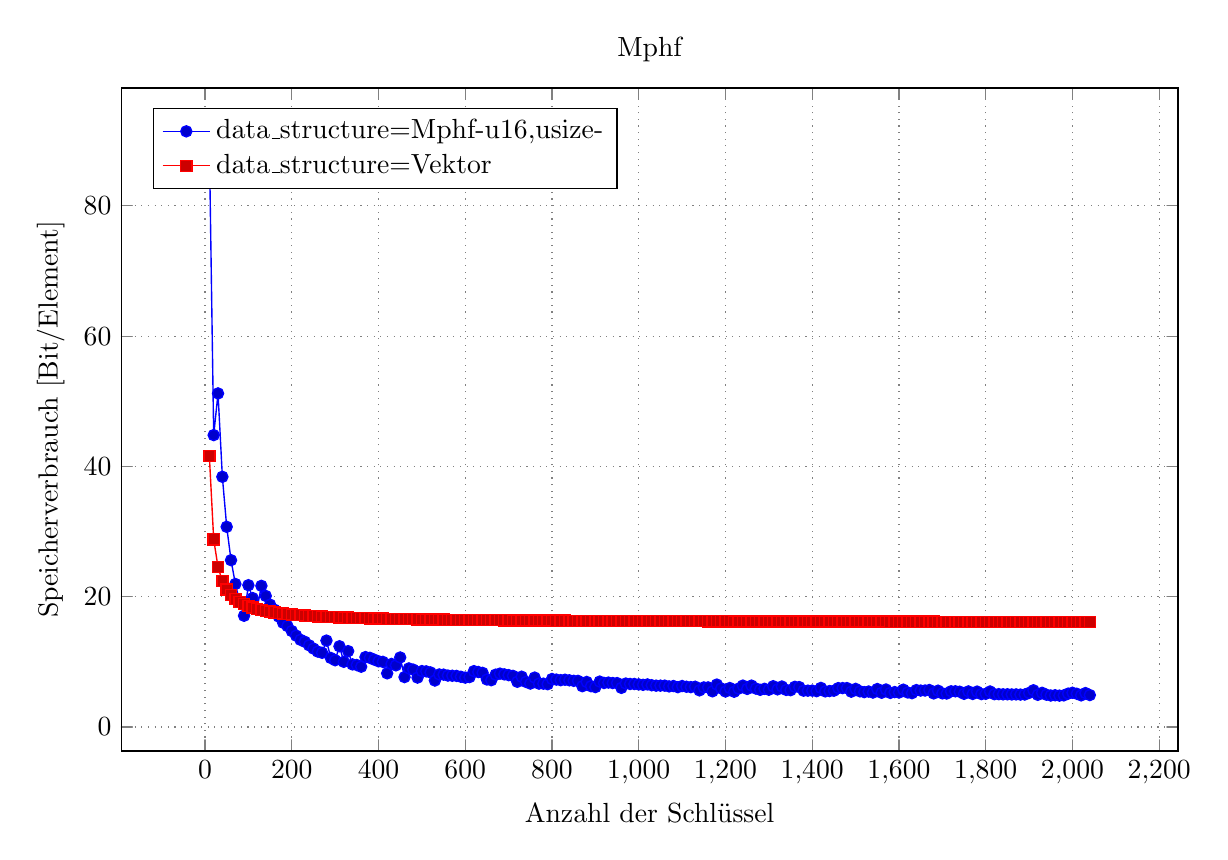
\begin{tikzpicture}
	\begin{axis}[
	title={Mphf},
	xlabel={Anzahl der Schlüssel},
	ylabel={Speicherverbrauch [Bit/Element]},
	]
	
	%% MULTIPLOT(data_structure) SELECT size AS x, size_bytes AS y, MULTIPLOT
	%% FROM mphf WHERE x % 10 == 0 GROUP BY MULTIPLOT,x ORDER BY MULTIPLOT,x
 \addplot coordinates { (10,89.6) (20,44.8) (30,51.2) (40,38.4) (50,30.72) (60,25.6) (70,21.9429) (80,19.2) (90,17.0667) (100,21.76) (110,19.7818) (120,18.1333) (130,21.6615) (140,20.1143) (150,18.7733) (160,18.0) (170,16.9412) (180,16.0) (190,15.4947) (200,14.72) (210,14.019) (220,13.3818) (230,13.0783) (240,12.5333) (250,12.032) (260,11.5692) (270,11.3778) (280,13.2571) (290,10.5931) (300,10.24) (310,12.3871) (320,10.0) (330,11.6364) (340,9.6) (350,9.50857) (360,9.24444) (370,10.7243) (380,10.6105) (390,10.3385) (400,10.08) (410,9.99024) (420,8.22857) (430,9.67442) (440,9.45455) (450,10.6667) (460,7.65217) (470,8.98723) (480,8.8) (490,7.57551) (500,8.576) (510,8.53333) (520,8.36923) (530,7.12453) (540,8.05926) (550,8.02909) (560,7.88571) (570,7.85965) (580,7.83448) (590,7.70169) (600,7.57333) (610,7.65902) (620,8.56774) (630,8.43175) (640,8.3) (650,7.28615) (660,7.17576) (670,8.02388) (680,8.18824) (690,8.06957) (700,7.95429) (710,7.84225) (720,6.93333) (730,7.71507) (740,6.91892) (750,6.656) (760,7.57895) (770,6.64935) (780,6.64615) (790,6.56203) (800,7.36) (810,7.26914) (820,7.18049) (830,7.24819) (840,7.1619) (850,7.07765) (860,7.06977) (870,6.25287) (880,6.90909) (890,6.25618) (900,6.11556) (910,6.96264) (920,6.74783) (930,6.8129) (940,6.74043) (950,6.73684) (960,6.0) (970,6.66392) (980,6.59592) (990,6.59394) (1000,6.528) (1010,6.46337) (1020,6.52549) (1030,6.4) (1040,6.33846) (1050,6.33905) (1060,6.33962) (1070,6.22056) (1080,6.28148) (1090,6.10642) (1100,6.28364) (1110,6.16937) (1120,6.11429) (1130,6.17345) (1140,5.61404) (1150,6.06609) (1160,6.06897) (1170,5.47009) (1180,6.50847) (1190,5.91597) (1200,5.44) (1210,5.97686) (1220,5.40328) (1230,5.87967) (1240,6.34839) (1250,5.8368) (1260,6.34921) (1270,5.89606) (1280,5.7) (1290,5.85426) (1300,5.71077) (1310,6.25344) (1320,5.7697) (1330,6.20752) (1340,5.68358) (1350,5.64148) (1360,6.16471) (1370,6.11971) (1380,5.56522) (1390,5.57122) (1400,5.57714) (1410,5.4922) (1420,5.99437) (1430,5.46014) (1440,5.51111) (1450,5.56138) (1460,5.96164) (1470,5.96463) (1480,5.96757) (1490,5.41208) (1500,5.84533) (1510,5.46755) (1520,5.34737) (1530,5.43791) (1540,5.27792) (1550,5.82194) (1560,5.25128) (1570,5.74777) (1580,5.22532) (1590,5.35346) (1600,5.28) (1610,5.72422) (1620,5.29383) (1630,5.18282) (1640,5.65854) (1650,5.58545) (1660,5.59036) (1670,5.67186) (1680,5.14286) (1690,5.56686) (1700,5.15765) (1710,5.12749) (1720,5.46977) (1730,5.47514) (1740,5.4069) (1750,5.08343) (1760,5.45455) (1770,5.06215) (1780,5.42921) (1790,5.04134) (1800,5.08444) (1810,5.4453) (1820,5.02857) (1830,5.03607) (1840,5.0087) (1850,5.01622) (1860,4.98925) (1870,4.99679) (1880,4.97021) (1890,4.97778) (1900,5.22105) (1910,5.62932) (1920,4.93333) (1930,5.23938) (1940,4.94845) (1950,4.82462) (1960,4.86531) (1970,4.80812) (1980,4.84848) (1990,5.11357) (2000,5.248) (2010,5.09453) (2020,4.84752) (2030,5.20197) (2040,4.89412) };
 \addlegendentry{data\_structure=Mphf-u16,usize-};
 \addplot coordinates { (10,41.6) (20,28.8) (30,24.5333) (40,22.4) (50,21.12) (60,20.2667) (70,19.6571) (80,19.2) (90,18.8444) (100,18.56) (110,18.3273) (120,18.1333) (130,17.9692) (140,17.8286) (150,17.7067) (160,17.6) (170,17.5059) (180,17.4222) (190,17.3474) (200,17.28) (210,17.219) (220,17.1636) (230,17.113) (240,17.0667) (250,17.024) (260,16.9846) (270,16.9481) (280,16.9143) (290,16.8828) (300,16.8533) (310,16.8258) (320,16.8) (330,16.7758) (340,16.7529) (350,16.7314) (360,16.7111) (370,16.6919) (380,16.6737) (390,16.6564) (400,16.64) (410,16.6244) (420,16.6095) (430,16.5953) (440,16.5818) (450,16.5689) (460,16.5565) (470,16.5447) (480,16.5333) (490,16.5224) (500,16.512) (510,16.502) (520,16.4923) (530,16.483) (540,16.4741) (550,16.4655) (560,16.4571) (570,16.4491) (580,16.4414) (590,16.4339) (600,16.4267) (610,16.4197) (620,16.4129) (630,16.4063) (640,16.4) (650,16.3938) (660,16.3879) (670,16.3821) (680,16.3765) (690,16.371) (700,16.3657) (710,16.3606) (720,16.3556) (730,16.3507) (740,16.3459) (750,16.3413) (760,16.3368) (770,16.3325) (780,16.3282) (790,16.3241) (800,16.32) (810,16.316) (820,16.3122) (830,16.3084) (840,16.3048) (850,16.3012) (860,16.2977) (870,16.2943) (880,16.2909) (890,16.2876) (900,16.2844) (910,16.2813) (920,16.2783) (930,16.2753) (940,16.2723) (950,16.2695) (960,16.2667) (970,16.2639) (980,16.2612) (990,16.2586) (1000,16.256) (1010,16.2535) (1020,16.251) (1030,16.2485) (1040,16.2462) (1050,16.2438) (1060,16.2415) (1070,16.2393) (1080,16.237) (1090,16.2349) (1100,16.2327) (1110,16.2306) (1120,16.2286) (1130,16.2265) (1140,16.2246) (1150,16.2226) (1160,16.2207) (1170,16.2188) (1180,16.2169) (1190,16.2151) (1200,16.2133) (1210,16.2116) (1220,16.2098) (1230,16.2081) (1240,16.2065) (1250,16.2048) (1260,16.2032) (1270,16.2016) (1280,16.2) (1290,16.1984) (1300,16.1969) (1310,16.1954) (1320,16.1939) (1330,16.1925) (1340,16.191) (1350,16.1896) (1360,16.1882) (1370,16.1869) (1380,16.1855) (1390,16.1842) (1400,16.1829) (1410,16.1816) (1420,16.1803) (1430,16.179) (1440,16.1778) (1450,16.1766) (1460,16.1753) (1470,16.1741) (1480,16.173) (1490,16.1718) (1500,16.1707) (1510,16.1695) (1520,16.1684) (1530,16.1673) (1540,16.1662) (1550,16.1652) (1560,16.1641) (1570,16.1631) (1580,16.162) (1590,16.161) (1600,16.16) (1610,16.159) (1620,16.158) (1630,16.1571) (1640,16.1561) (1650,16.1552) (1660,16.1542) (1670,16.1533) (1680,16.1524) (1690,16.1515) (1700,16.1506) (1710,16.1497) (1720,16.1488) (1730,16.148) (1740,16.1471) (1750,16.1463) (1760,16.1455) (1770,16.1446) (1780,16.1438) (1790,16.143) (1800,16.1422) (1810,16.1414) (1820,16.1407) (1830,16.1399) (1840,16.1391) (1850,16.1384) (1860,16.1376) (1870,16.1369) (1880,16.1362) (1890,16.1354) (1900,16.1347) (1910,16.134) (1920,16.1333) (1930,16.1326) (1940,16.132) (1950,16.1313) (1960,16.1306) (1970,16.1299) (1980,16.1293) (1990,16.1286) (2000,16.128) (2010,16.1274) (2020,16.1267) (2030,16.1261) (2040,16.1255) };
 \addlegendentry{data\_structure=Vektor};
 
 
	
	\end{axis}
	\end{tikzpicture}
\end{center}




\end{document}

%%%%%%%%%%%%%%%%%%%%%%%%%%%%%%%%%%%%%%%%%%%%%%%%%%%%%%%%%%%%%%%%%%%%%%%%%%%%%%%%
